\documentclass{article}

\def\npart {II}
\def\nyear {2017}
\def\nterm {Michaelmas}
\def\nlecturer{Dr H.\ Krieger}
\def\ncourse{Riemann Surfaces}
\def\draft{Incomplete}
\ifx \nauthor\undefined
  \def\nauthor{Bhavik Mehta}
\else
\fi

\author{Based on lectures by \nlecturer \\\small Notes taken by \nauthor}
\date{\nterm\ \nyear}
\title{Part \npart\ -- \ncourse}

\usepackage[utf8]{inputenc}
\usepackage{amsmath}
\usepackage{amsthm}
\usepackage{amssymb}
\usepackage{enumerate}
\usepackage{mathtools}
\usepackage{graphicx}
\usepackage[dvipsnames]{xcolor}
\usepackage{tikz}
\usepackage{wrapfig}
\usepackage{centernot}
\usepackage{float}
\usepackage{braket}
\usepackage[hypcap=true]{caption}
\usepackage{enumitem}
\usepackage[colorlinks=true, linkcolor=mblue]{hyperref}
\usepackage[nameinlink,noabbrev]{cleveref}
\usepackage{nameref}
\usepackage[margin=1.5in]{geometry}

% Theorems
\theoremstyle{definition}
\newtheorem*{aim}{Aim}
\newtheorem*{axiom}{Axiom}
\newtheorem*{claim}{Claim}
\newtheorem*{cor}{Corollary}
\newtheorem*{conjecture}{Conjecture}
\newtheorem*{defi}{Definition}
\newtheorem*{eg}{Example}
\newtheorem*{ex}{Exercise}
\newtheorem*{fact}{Fact}
\newtheorem*{law}{Law}
\newtheorem*{lemma}{Lemma}
\newtheorem*{notation}{Notation}
\newtheorem*{prop}{Proposition}
\newtheorem*{question}{Question}
\newtheorem*{rrule}{Rule}
\newtheorem*{thm}{Theorem}
\newtheorem*{assumption}{Assumption}

\newtheorem*{remark}{Remark}
\newtheorem*{warning}{Warning}
\newtheorem*{exercise}{Exercise}

% \newcommand{\nthmautorefname}{Theorem}

\newtheorem{nthm}{Theorem}[section]
\newtheorem{nlemma}[nthm]{Lemma}
\newtheorem{nprop}[nthm]{Proposition}
\newtheorem{ncor}[nthm]{Corollary}
\newtheorem{ndef}[nthm]{Definition}

% Special sets
\newcommand{\C}{\mathbb{C}}
\newcommand{\N}{\mathbb{N}}
\newcommand{\Q}{\mathbb{Q}}
\newcommand{\R}{\mathbb{R}}
\newcommand{\Z}{\mathbb{Z}}

\newcommand{\abs}[1]{\left\lvert #1\right\rvert}
\newcommand{\norm}[1]{\left\lVert #1\right\rVert}
\renewcommand{\vec}[1]{\boldsymbol{\mathbf{#1}}}

\let\Im\relax
\let\Re\relax

\DeclareMathOperator{\Im}{Im}
\DeclareMathOperator{\Re}{Re}
\DeclareMathOperator{\id}{id}

\definecolor{mblue}{rgb}{0., 0.05, 0.6}


% preamble
\setcounter{section}{-1}
\usetikzlibrary{cd}
% and here we go!

\begin{document}
\maketitle

\section{Complex analysis and complex log}

\begin{defi}
    A smooth function $f: U \to \C$ (where $U$ is a domain in $\C$) is \textbf{holomorphic} or \textbf{analytic} if either of the following equivalent statements hold:
    \begin{enumerate}[label=(\arabic*)]
        \item $f$ is differentiable at all points of $U$, where differentiability is defined by limits, and checked by the Cauchy-Riemann equations
        \item $\forall a \in U$, $f$ has a power series expansion on a neighbourhood of $a$:
            \begin{equation*}
                f(z) = \sum_{n \geq 0} a_n (z - a)^n
            \end{equation*}
            and the series converges on some disk about $a$ with positive radius.
    \end{enumerate}
\end{defi}
\begin{proof}[Sketch of proof of equivalence]

    \leavevmode

    $(\Rightarrow)$ Use the Cauchy Integral Formula to construct $a_n$, and convergence.

    $(\Leftarrow)$ Show directly that the term-by-term derivative exists, and that it agrees with the limit definition of the derivative.
\end{proof}

Note that a power series tells you about local behaviour.
If $f(z)$ is not identically zero near $a \in U$, there exists some minimal $n_0$ such that $a_{n_0} \neq 0$.
We can write $f$ locally as
\begin{align*}
    f(z) &= a_{n_0} (z-a)^{n_0} + \sum_{n \ge n_0} a_n (z-a)^n \\
         &= a_{n_0} (z-a)^{n_0} \left(1 + \sum_{n>n_0} \frac{a_n}{a_{n_0}} (z-a)^{n-n_0}\right)
\end{align*}
As $z \to a$, the sum $\to 0$ so the quantity in the brackets tends to 1.  So, $f(z) = a_{n_0} (z-a)^{n_0} g(z)$, where $g$ is analytic and nonzero on a neighbourhood of $a$.
Consequently, we have the \emph{principle of isolated zeros}: for $f$ analytic on domain $U$, then for all $a \in U$ such that $f(a) = 0$, either $f$ is identically $0$ on a neighbourhood of $a$, or $f$ is never $0$ on a punctured disk centred at $a$.  But recall a domain refers to an open \emph{and connected} set.  So, if $f$ is identically $0$ (improve this writing) on a neighbourhood of $a$, call it $D_a$.  If $f \ne 0$ on a punctured disk about $a$, call it $P_a^*$. Construct
\begin{align}
    V = \bigcup_{\substack{a \in U \text{such that} \\ f \equiv 0 \text{on a neighbourhood of} a}} D_a
    % W = \cup_{a \in U such that f \ne 0 on a punctured neighbourhood of a} P_a^*
\end{align}

$V$ and $W$ are open, disjoint and $V \cup W = U$. Since $U$ is connected, $U=V$ or $U=W$. So either $f \equiv 0$ on $U$, or $f$ has only isolated zeros.
This will both be referred to as the principle of isolated zeros.

(corollary) (identity principle)
If $f$ and $g$ are analytic on $U$, then either $f \equiv g$ on $U$, or ${z \in U : f(z) = g(z)}$ consists of isolated points.
Proof (clear)

(definition)
If f is analytic on a punctured disk $\mathbb{D}^*(a,r)$, then we say $a$ is an isolated singularity of $f$.
If so, then there exists a Laurent expansion $\sum_{n=-\infty}^{\infty} a_n (z-a)^n$ near $a$, which come in three types.

I. Removable singularity. $f$ extends to an analytic function on $\mathbb{D}^*{a, r}$. Phrased in terms of Laurent expansions, $a_n = 0 \forall n < 0$.
(thm) (Removable singularities theorem) $f$ has a removable singularity at $a$ if and only if $f$ is bounded on a punctured neighbourhood about $a$.
(proof sketch) (=>) follows from continuity of analytic functions
(<=) Cauchy's theorem and integral formula still hold for punctured neighbourhoods so long as $f(z) (z-a) \to 0$ as $z \to a$.  With a small circle about $a$, we can show directly that $a_n = 0$ for $n < 0$.

II. Poles: $f$ has a pole at $a$ if $a_n = 0$ for all $n < n_0$ for some $n_0$. Locally, this occurs if and only if $|f(z)| \to \infty$ as $z \to a$ (using the Laurent series).

III. Essential singularity: $a_n \neq 0$ for finitely many $n < 0$, f has an essential singularity at $a$.
thm [Casorati-Weierstrass] If $f$ has an essential singularity at $a$, then the image of $f$ on any punctured neighbourhood of $a$ is dense in $\mathbb{C}$.
(proof sketch) Examine $\frac1{f(z) - \gamma}$ if the image of $f$ misses a neighbourhood of $\gamma$.

\paragraph{Examples}
$f(z) = \frac1{e^z - 1}$ has poles wherever $e^z = 1$.
At $\infty$, we also have an isolated singularity, recalling that punctured neighbourhoods of $\infty$ are $\mathbb{C}\\ \mathbb{D}(0, R)$. Since $e^z$ takes all nonzero values or strips of $\mathbb{C}$, we cannot have $e^z \to 1$ as $z \to \infty$, hence $f$ cannot have a pole.  On the other hand, there exists arbitrarily large solutions (in modulus) to $e^z = 1$, and $f$ cannot have a removable singularity at $\infty$.  Hence, this singularity is essential.

(edit: not isolated as every neighbourhood of infinity contains a singularity)

\subsection{Complex logarithm}
The complex logarithm is an example of a multivalued function, which arises as the inverse of an analytic function. Given nonzero $z$, if $e^w = z$, $z = r e^{i \theta}$, then $w = \log r + (2 \pi n + \theta i)$ for some $n \in \mathbb{Z}$.  We cannot make a continuous choice of $n$ on all of $\mathbb{C}$, so we define the complex log on domains like $\mathbb{C} \\ \mathbb{R}_{\leq 0} =: U$. We have for each $n$, a choice of logarithm which can be analytically defined on $U$.  Recall a \emph{continuous} inverse of an analytic function is analytic.

% Lecture 2

Let $U_1 = \C \setminus \R_{\geq 0}$.

\begin{prop}
    For $n \in \Z$, define $h(z)$ on $U$, by
    \begin{equation*}
        h(z) = \int_{-1}^z \frac{dw}{w} + (2n+1) \pi i
    \end{equation*}
    with integral along straight line joining $-1$ and $z$.

    Then $h$ is analytic on $U_1$ and is the inverse to the exponential function on $U_1$.
\end{prop}

\begin{proof}
    Let $z \in U_1$. $\tau \in \C$ with $\abs{\tau}$ sufficiently small, such that the triangle is entirely in the domain.

    Then claim $\frac{h(z + \tau) - h(z)}{\tau} = \frac1{\tau} \int_z^{z+\tau} \frac{dw}{w} \to \frac1z$.
    The first equality follows from Cauchy's theorem, since $h$ is continuous in the triangle.

    \begin{align*}
        \abs{\frac{1}{\tau} \int_z^{z + \tau} \frac{dw}{w} - \frac12} &= \abs{\frac1{\tau} \int_z^{z+\tau} \frac{z-w}{zw} dw} \\
        &\leq C \tau \to 0
    \end{align*}


    Thus $h$ is analytic on $U_1$, with $h'(z) = \frac{1}{z}$.

    Look at $g(z) = \frac{e^{h(z)}}{z}$, so $g'(z) = \frac{z h'(z) e^{h(z)} - e^{h(z)}}{z^2} = 0$, thus $g$ is constant. But, we still need to find out what it's value us, so consider $g(-1)$. $g(-1) = \frac{e^{h(-1)}}{-1} = -e^{(2n+1) \pi i} = 1$.
    Thus, $e^{h(z)} \equiv z$ on $U_1$, so $h$ is the inverse to the exponential.
\end{proof}

\begin{remark}
    We can't extend the function $H$ continuously across the positive real axis.
\end{remark}

\subsection{Analytic continuation}
Fix a domain $U \in \C$ which is path connected.

\begin{defi}[\hypertarget{def:directAnalCont}{Direct Analytic Continuation}]
    A \textbf{function element} (or \textbf{function germ}) on $U$ is a pair, $(f, D)$ where $f$ is analytic on the domain $D \subseteq U$.

    Two function elements $(f, D)$ and $g, E)$ are \textbf{equivalent} if $D \cap E \neq \emptyset$ and $f = g$ on $D \cap E$. In this case, we say $(g, E)$ is a \textbf{direct analytic continuation} of $(f, D)$.
\end{defi}

\begin{remark}
    This is not an equivalence relation.  In the diagram, $(f_1, D_1)$ and $(f_3, D_3)$ are not equivalent since $D_1 \cap D_3 = \emptyset$.
\end{remark}
% why do they do this to me :(

\begin{defi}[\hypertarget{def:pathAnalCont}{Analytic continuation along a path}]
    We say $(g, E)$ is an analytic continuation of $(f, D)$ along a path $\gamma: [0, 1] \to U$, written as $(f, D) \sim_\gamma (g, E)$.  If there exists $(f_1, D_1), \dotsc, (f_n, D_n)$ and $0 = t_0 < t_1 < \dots < t_n = 1$ with $\gamma([t_{i-1}, t_i]) \subseteq D_i$ for $1 \leq i \leq n$ and $(f_1, D_1) = (f, D)$, $(f_n, D_n) = (g, E)$ and $(F_{i-1}, D_{i-1}) \sim (F_i, D_i)$, that is $(f_i, D_i)$ is a \hyperlink{def:directAnalCont}{direct analytic continuation} of $f_{i-1}, D_{i-1}$.
\end{defi}


\begin{defi}[\hypertarget{def:analCont}{Analytic continuation}]
    We say $(g, E)$ is an analytic continuation of $(f, D)$ if there exists a path $\gamma$ with $(f, D) \sim_\gamma (g, E)$.  We write $(f, D) \approx (g, E)$.
\end{defi}

\begin{remark}
    $\approx$ is an equivalence relation.  Reflexivity and symmetry are easy, and transitivity can be seen from the diagram.
\end{remark}


\begin{defi}
    An equivalence class $\mathcal{F}$ under $\approx$ is a \textbf{complete analytic function}.
\end{defi}

\begin{eg}
    Set $U = \C^* = \C \setminus {0}$.  Fix $(\alpha, \beta) \subseteq \R$, with $\abs{\beta-\alpha} \leq 2 \pi$, and define
    \begin{equation*}E_{\alpha, \beta} = \set{z = r e^{i \theta} | \alpha < \theta < \beta \, , \; r > 0}\end{equation*}
    So we can see $U_1 = E_(0, 2 \pi)$.
    Define $f_{(\alpha, \beta)} : E_{(\alpha, \beta)} \to \C$ by $f_{(\alpha, \beta)} (r e^{i \theta}) = \log r + i \theta$, $\theta \in (\alpha, \beta)$.

    Write $L_{(\alpha, \beta)}$ for the function element $(f_{(\alpha, \beta)}, E_{(\alpha, \beta)})$.

    Consider the three function elements $L_{-\frac\pi2, \frac\pi2}$, $L_{\frac\pi6, \frac{7\pi}6}$, $L_{\frac{5\pi}6, \frac{11\pi}{6}}$
    We can see the direct analytic continuations, but we do not have direct analytic continuation (), but ().
\end{eg}

\begin{aim}
    Construct a surface on which $\log$ is well-defined by gluing together a bunch of domains on which it is well-defined.
\end{aim}

For each $n \in \Z$, take a copy of $U_1 = E_{(0, 2\pi)}$.  Each has a well-defined choice of logarithm: $f_{(2\pi n, 2\pi (n+1))}$, $r e^{i \theta} \mapsto \log r + (\theta + 2 \pi n) i$, for $\theta \in (0, 2\pi)$.

We can glue together these copies of $U$, so that the functions $f_{(2\pi n, 2\pi (n+1))}$ glue to give a continuous function $L : \tilde{U} \to \C$.

\begin{defi}[{Covering map}\hypertarget{def:coverMap}]
    A \textbf{covering map} of a topological space $X$ is is (sic) a continuous map $\pi: \widetilde X \to X$, where $\widetilde X$ and $X$ are Hausdorff and path connected, and $\pi$ is a local homeomorphism.  Specifically, $\forall \widetilde x \in \widetilde X$, $\exists$ an open neighbourhood $\widetilde N$ of $\widetilde{x}$ on which $\pi$ restricts to a homeomorphism.
    We say that $X$ is the \textbf{base space} of $\pi$.
\end{defi}
Note that this is likely weaker than the definition used in Algebraic Topology, which requires that $\forall x \in X$, $\exists$ an open neighbourhood $N$ of $x$ such that $\pi^{-1}(N)$ is a disjoint union of open sets which are mapped homeomorphically by $\pi$ to $N$.  We will call this a \textbf{regular} covering map.

\begin{eg}
    Non-regular covering map: Consider $\pi(z) = e^z$ on the domain
    \begin{equation}
        \set{z | 0 < \Im(z) < 4\pi}
    \end{equation}

    Let $x = 1$.  From the diagram, we have a disjoint union of open neighbourhoods, but $\pi$ does not map them homeomorphically.
\end{eg}

Define $R \coloneqq \sqcup_{n\in \Z} \C^* \times {n}$, and equip $R$ with the topology from basis with elements of the two forms:
\begin{enumerate}
    \item for $(\eta, n) \in R$ with $\eta \notin \R_{\leq 0}$ and any $r>0$, such that $\mathbb{D}(\eta, r) \cap \mathbb{R}_{\leq 0} = \emptyset$, define an open set $D((\eta, n), r)$ to be the disk of radius $r$ about $\eta$ in the $n$th sheet:
        \begin{equation}
            D((\eta, n), r) \coloneqq \set{(z, n) | \abs{z - \eta} < r}
        \end{equation}

    \item For $(\eta, n)$ with $\eta \in \R_{\leq 0}$, define
        \begin{equation}
            A((\eta, n), r) \coloneqq \set{(z, n) | \abs{z - \eta} < r, \ \Im{z} \geq 0} \sqcup {(z, n-1) | \abs{z - \eta} < r, \ \Im{z} < 0}
        \end{equation}
        where $r < \abs{\eta}$
\end{enumerate}

This defines a path-connected, Hausdorff topology on $R$. The map $\pi: \R \to \C^*$ given by $\pi((z, n)) = z$ is a (regular) covering map. Define $f:R \to \C$ by $f(r e^{i \theta}, n) = \log r + i (2 \pi n + \theta)$ where $\theta \in [0, 2\pi)$. By construction, $f$ is continuous, $f$ is also a bijection, and (diagram).
In this sense, $f$ is a logarithm.

Note we can similarly construct a gluing spae for $z^{1/n}$ as a multivalued function, $z^{1/n} = r^{1/n} e^{i \theta/n} e^{2 \pi k i/n}$ so the $n$th sheet glues to the first.
This is a regular covering map, but only because $0$ is not included.

\subsection{Power series and continuation}
Recall a power series is absolutely and uniformly convergent on any closed disk inside its radius of convergence. If that radius of convergence is not $\infty$, what can we say about how far the series can be analytically continued? Without loss of generality assume we are working on the unit disk $\mathbb{D}$, that is a series about zero and radius of convergence $1$.  We denote $\mathbb{T} \coloneqq \partial \mathbb{D}$ and write $f(z) = \sum_{k \geq 0} a_k z^k$.

\begin{defi}
    We say that $z \in \mathbb{T}$ is \textbf{regular} if $\exists$ an open disk $N$ about $z$ and an analytic function $g$ on $N$ such that $f = g$ on $N \cap \mathbb{D}$. If $z$ is not regular, it is \textbf{singular}.
\end{defi}

Note the collection of regular points is open, and the collection of singular points is closed.

Warning: regularity is independent of series convergence!
\begin{enumerate}[label=(\arabic*)]
    \item $f(z) \coloneqq \sum_{k \geq 0} z^k$. This doesn't converge anywhere on $\mathbb{T}$, but as it agrees with $\frac1{1-z}$, all points except $z=1$ are regular.
    \item
        \begin{equation}
            g(z) \coloneqq \sum_{k=2}^\infty \frac{z^k}{k(k-1)}
        \end{equation}
        converges on $\mathbb{T}$ but $1$ is a singular point, as if $g$ extends analytically to a neighbourhood of $1$, so $g''$ does also, a contradiction.
\end{enumerate}

\begin{prop}
    If $f(z) = \sum a_k z^k$ has radius of convergence $1$, then $\exists$ singular point on $\mathbb{T}$.
\end{prop}

\begin{proof}
    Suppose not, then for each $z \in \mathbb{T}$, $\exists D_z$ and analytic $g_z$ on $D_z$ with $f = g_z$ on $D_z \cap \mathbb{D}$. Given $z_1 \neq z_2$ on $\mathbb{T}$ with $D_{z_!} \cap D_{z_2} \neq \emptyset$, then since these are disks centered at points of $\mathbb{T}$, $D_{z_1} \cap D_{z_2} \cap \mathbb{D} \neq \emptyset$, so $f = g_{z_1} = g_{z_2}$ on $\mathbb{D} \cap D_{z_1} \cap D_{z_2}$. By the identity principle $g_{z_1} = g_{z_2}$ on $D_{z_1} \cap D_{z_2}$, as $\mathbb{T}$ is compact, it many be covered by finitely many of these disks, so $f$ can be extended to the union $\mathbb{D}$ with this finite collection of $D_z$, and that union contains $\mathbb{D}(0, 1 + \delta)$ for some $\delta > 0$, contradiction.
\end{proof}

\begin{defi}
    We say $\mathbb{T}$ is a \textbf{natural boundary} of $f$ if every point $z \in \mathbb{T}$ is singular.
\end{defi}

\begin{eg}
    $f(z) \coloneqq \sum_{k=0}^\infty z^{k!}$. Let $\omega$ be a root of unity, $\omega = e^{2 \pi i p/q}$.
    Then
    \begin{align*}
        f(r e^{2\pi i p/q}) &= \sum_{k=0}^\infty r^{k!} (e^{2 \pi i p/q})^{k!} \\
                            &= \underbracket{\sum_{k=0}^{q-1} r^{k!} (e^{2 \pi i p/q})^{k!}}_{\text{bounded as} \; r \to 1} + \underbracket{\sum_{k=q}^\infty r^{k!}}_{\text{approaches} \; \infty \; \text{as} \; r \to 1}
    \end{align*}

    But
\end{eg}

\begin{center}
    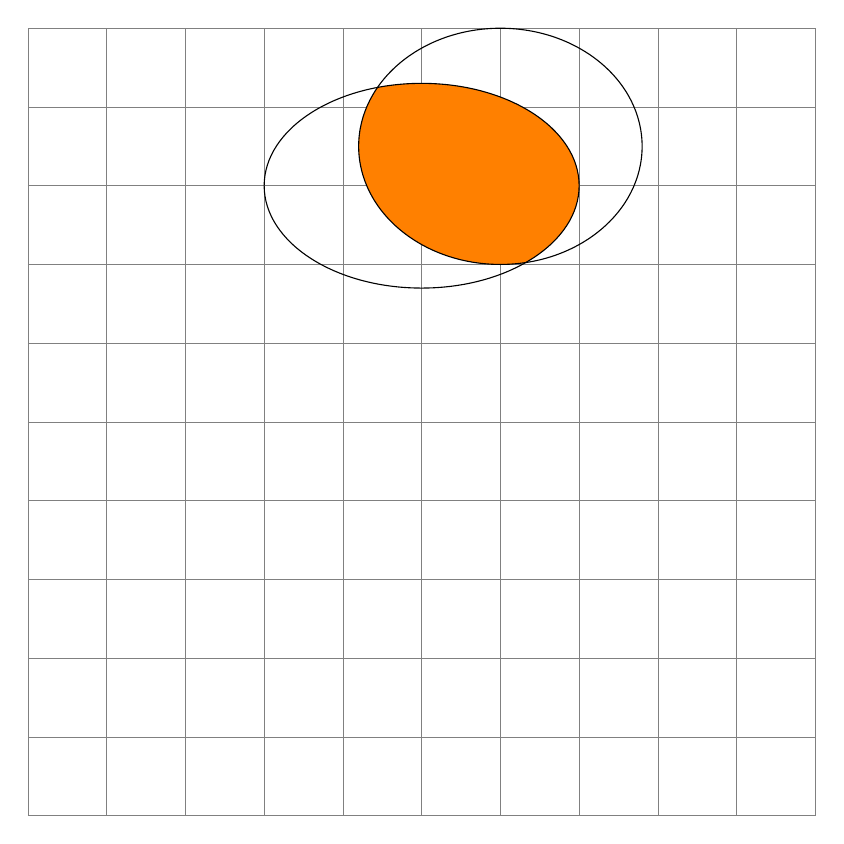
\begin{tikzpicture}
        \draw[help lines] (-5, -5) grid (5, 5);
        \begin{scope}
            \clip (0, 3) ellipse (2cm and 1.3cm);
            \fill[orange] (1, 3.5) ellipse (1.8cm and 1.5cm);
        \end{scope}
        \draw (1, 3.5) ellipse (1.8cm and 1.5cm);
        \draw (0, 3) ellipse (2cm and 1.3cm);
    \end{tikzpicture}
\end{center}

\begin{defi}\hypertarget{def:rs}
    A \textbf{Riemann surface} is a connected, Hausdorff topological space $R$, together with a collection of open subsets $\mathcal{U}_\alpha \subset \R$ and homeomorphisms $\phi_\alpha:\mathcal{U}_\alpha\to D_\alpha$, where $D_\alpha$ is an open subset of $\C$ satisfying
    \begin{enumerate}
        \item
            $ \bigcup_\alpha \mathcal{U}_\alpha = R $
        \item for any $\alpha, \beta$ with $\mathcal{U}_\alpha \cap \mathcal{U}_\beta \neq \emptyset$, then the map
            \begin{equation*}
                \phi_\alpha \circ \phi_\beta^{-1}: \phi_{\beta}(\mathcal{U}_\alpha \cap \mathcal{U}_\beta) \to D_{\alpha}
            \end{equation*}
            is analytic as a map of open sets in $\C$.
    \end{enumerate}

    The information $(\mathcal{U}_\alpha, \phi_\alpha)$ is called a \textbf{chart} of $R$.
    The compositions $\phi_\alpha \circ \phi_{\beta}^{-1}$ are the \textbf{transition functions} of $R$.
    The collection of charts $\{U_\alpha, \phi_\alpha\}$ is the \textbf{atlas} of $R$.
\end{defi}

\begin{remark}
    \leavevmode
    \begin{enumerate}
        \item As transitions are invertible with analytic inverses, they are conformal equivalences.
        \item $R$ is path connected as it is connected and locally path connected

            Fix $z_0 \in R$. Define $U = \set{z \in R \mid \exists\text{path from } z_0 \text{ to } z}$. $U$ is open, as it its complement. As $R$ is connected, $U^c$ is empty.
        \item Occasionally, `connected' will not be included in the definition, but this can be annoying without limiting the number of connected components.
    \end{enumerate}
\end{remark}

\begin{eg}
    $\C$ as a topological space, for instance $(\C, \phi(z) = z)$, $(\C, \phi(z) = z+1)$, $(\C, \phi(z) = \bar{z})$.
\end{eg}

\begin{defi}
    Let $R$ be a \hyperlink{def:rs}{Riemann surface}.
    Two atlases $\{(\mathcal{U}_\alpha, \phi_\alpha)\}$, $\{(\mathcal{U}_\beta, \psi_\beta)\}$ are \textbf{equivalent} if their refinement $\{(\mathcal{U}_\beta, \phi_\beta)\} \cup \{(\mathcal{U}_\beta, \psi_\beta)\}$ is an atlas. In other words,
    \begin{equation}
        \psi_\beta \circ \phi_\alpha^{-1}: \phi_\alpha(\mathcal{U}_\alpha \cap V_\beta) \to \psi_\beta(\mathcal{U}_\alpha \cap V_\beta)
    \end{equation}
    is analytic (and similarly for $\phi_\alpha \circ \psi_\beta^{-1}$).
\end{defi}
This defines an equivalence relation, as we will soon see.

\begin{eg}
    $(\C, \phi(z) = z)$, $(\C, \phi(z) = z+1)$: the refinement has transition maps: identity, $z \mapsto z+1$, $z \mapsto z-1$, so these are equivalent atlases.
    Non-example:
    $(\C, \phi(z) = z)$, $(\C, \phi(z) = \bar{z})$, the transition functions of the refinement are identity and complex conjugation, so these are \emph{not} equivalent atlases.
\end{eg}

\begin{defi}
    We call an equivalence class of atlases a \textbf{conformal structure} on $R$.
\end{defi}
\begin{remark}
    \begin{enumerate}
        \item We could have defined a Riemann surface as a connected Hausdorff topological space which admits a conformal structure.
        \item If $S \subset R$ is open, connected then $R$ a Riemann surface implies $S$ a Riemann surface via restriction of charts.
    \end{enumerate}
\end{remark}

\begin{defi}
    Let $R, S$ be Riemann surfaces with atlases $\{(\mathcal{U}_\alpha, \phi_\alpha)\}, \{(\mathcal{U}_\beta, \psi_\beta)\}$ respectively, We say a map $f: R \to S$ is analytic if it is continuous and if for any $\mathcal{U}_\alpha cap f^{-1}(V \beta) \neq \emptyset$, the map
    \begin{equation}
        \psi_\beta \circ f \circ \phi_\alpha^{-1}: \phi_\alpha(\mathcal{U}_\alpha \cap f^{-1}(V_\beta)) \to \psi_\beta(f(\mathcal{U}_\alpha \cap f^{-1}(V_\beta)))
    \end{equation}
    is analytic.
\end{defi}

\begin{defi}
    An analytic map $f: R \to S$ of Riemann surfaces is a \textbf{conformal equivalence} (biholomorphism or analytic isomorphism) if $\exists$analytic inverse $g:S \to R$ of $f$.
\end{defi}

\begin{eg}
    We saw that $(\C, \phi(z) = z)$ and $(\C, \psi(z) = \bar{z})$ are inequivalent atlases, ie, define different conformal structures on $\mathcal{C}$. However, $f:(\C, \phi(z) = z) \to (\C, \psi(z) = \bar{z})$ given by $z \mapsto \bar{z}$ is a conformal equivalence of these two Riemann surfaces as the functions $(\psi \circ f \circ \phi^{-1})(z) = \bar{\bar{z}} = z$ are conformal isomorphisms.
\end{eg}

\begin{lemma}
    The composition of analytic maps $f: R\to S$ and $g: S \to T$ of Riemann surfaces is analytic.
\end{lemma}

We need for any $\gamma, \alpha$ with $\mathcal{U}_\alpha \cap h^{-1}(W_\gamma)$ that $\theta_\gamma \circ h \circ \phi_\alpha^{-1}$ is analytic on $\phi_\alpha(\mathcal{U}_\alpha \cap h^{-1}(W_\gamma))$.
In this set, analyticity is local, so it suffices to show that for any $\beta$ with $f^{-1}(V_\beta) \cap \mathcal{U}_\alpha \cap h^{-1}(W_\gamma) \neq \emptyset$, we have $\theta_\gamma \circ h \circ \phi_\alpha^{-1} \mid_{\phi_\alpha(\mathcal{U}_\alpha \cap h^{-1}(W_\gamma))}$ analytic on $\phi_\alpha()$.

\begin{cor}
    Equivalence of atlases is an equivalence relation.
\end{cor}

\begin{proof}
    Atlases $a_1$ and $a_2$ are equivalent by definition if the identity map $(R, a_1) \xrightarrow{\id} (R, a_2)$ is analytic. Reflexivity and symmetry are immediate, and transitivity follows from the previous lemma.
\end{proof}

\begin{prop}
    Let $R$ be a Riemann Surface and $\pi: \widetilde{R} \to R$ a covering map. Then $\exists!$conformal structure on $\widetilde{R}$ for which $\pi$ is analytic.
\end{prop}

\begin{proof}
    Given $z \in \widetilde{R}$, $\exists$neighbourhood $\widetilde{N_z}$ of $z$ such that $\pi$ is homeomorphic on $\widetilde{N_z}$.
    $\pi(z) \in U$ for some chart neighbourhood $\mathcal{U}$; $\pi(\widetilde{N}) \cap \mathcal{U}$ is open in $R$, so define $V \coloneqq \pi^{-1}(U) \cap \widetilde{N}$, an open set in $\widetilde{R}$.
    Define $\psi: V \to \C$ to be $\phi \circ \pi$, we obtain an atlas on $\widetilde{R}$, $\pi$ is analytic as the composition functions are just the transitions of the atlas on $R$.
    So $\exists$conformal structure on $\widetilde{R}$ for which $\pi$ is analytic, call this atlas $a$.
    Suppose $\exists a^*$ on $\widetilde{R}$ for which $\pi$ is analytic; we will show these atlases are equivalent.

    Say $(W, \theta)$ is a chart of $a^*$ and $z \in W$, find $(V, \psi)$ (and $\widetilde{N}$ and $\mathcal{U}$) as above.
    We assumed that $\pi$ is analytic for this atlas. As $\pi$ is analytic, $\phi \circ \pi \circ \theta^{-1}$ is analytic; it is also a homeomorphism, so its inverse is also analytic.
    So both types of transitions are analytic and the atlases are equivalent.
\end{proof}

\begin{equation*}
    \begin{tikzcd}
        R \arrow[r, "f"] \arrow[d, "\pi"] & \C \arrow[ld, "\exp"]\\
        \C^*
    \end{tikzcd}
\end{equation*}
As a corollary, we see that the gluing surface $R$ we constructed for $\log$ gives a conformal structure on $R$ for which $\pi$ is analytic.
Note $f$ is continuous by the open mapping theorem. It follows that $f$ is analytic (looking locally) but $f$ is a bijection. So $f$ has an analytic inverse, because the inverse is continuous. So $R$ is conformally equivalent to $\C$.

\begin{eg}
    The Riemann sphere.
    Let $\C_\infty \coloneqq \C \cup \{\infty\}$, equipped with the topology whose open sets are of the form: open subset of $\C$ or $\{\infty\} \cup \C \setminus K$ where $K \subseteq \C$ is compact.
    With this topology, $\C_\infty$ is homeomorphic to $S^2$ via stereographic projection and $\pi((0, 0, 1)) = \infty$.
    $C_\infty$ is connected, Hausdorff and compact.
    Define the atlas via two charts: $(\C: \phi(z) = z)$ and $(\C_\infty \setminus \{0\}, \phi(z) = \frac{1}{z})$.
    The transitions $\frac{1}{z}$ are analytic on $\C^*$.

    \begin{center}
        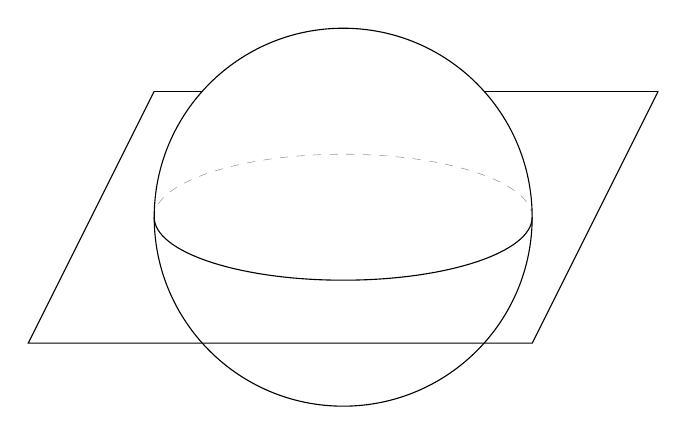
\begin{tikzpicture}[scale=0.8]
            % \draw[help lines] (-5, -5) grid (5, 5);
            \draw (5, 2) -- (-3, 2);
            \draw[fill=white] (0,0) circle [radius=3];
            \draw (3,0) arc [x radius=3, y radius=1, start angle=0, end angle=-180];
            \draw[opacity=0.4, very thin, dashed] (3,0) arc [x radius=3, y radius=1, start angle=0, end angle=180];
            \draw (-3, 2) -- (-5, -2) -- (3, -2) -- (5, 2);
        \end{tikzpicture}
    \end{center}
\end{eg}

\begin{defi}
    We define the Riemann Sphere as the above surface.
\end{defi}

\begin{defi}
    If $R$ is a Riemann surface, an analytic map $R \to \C$ is an analytic function: in terms of charts, if $(\mathcal{U}, \phi)$ is a chart for $R$, this required $f \circ \phi^{-1}$ is analytic.
\end{defi}

\begin{thm}[Inverse function theorem]
    Given $g$ analytic on an open set $V \subseteq \C$, and $a \in V$ with $g'(a) \neq 0$, $\exists$neighbourhood $N$ of $a$, $N \subseteq V$ such that $g|_N: N \to g(N)$ is a conformal equivalence.
\end{thm}

\begin{proof}
    Replace $g$ with $g(z) - g(a)$ to assume without loss of generality that $g(a) = 0$.
    Take a disk $\mathbb{D}(a, \epsilon)$ with $\\mathbb{D}(a, \epsilon) \subseteq V$ on which $a$ is the only zero of $g$, assume also $g'(z) \neq 0$ on $\overline{\mathbb{D}(a, \epsilon)}$.
    The argument principle tells us: if $\gamma$ is positively oriented disk boundary, then $n(g \circ \gamma, 0) =$ number of zeros of $g$ in the disk $ = 1$.
    $g \circ \gamma$ is compact so closed, so choose a disk $\Delta$ centred at 0 with $\Delta \cap (g \circ \gamma) = \emptyset$.

    For all $w \in \Delta$, $n(g \circ \gamma, w) = 1$ so let $N = g^{-1} (\Delta)$.
    Then $N$ is an open neighbourhood of $a$, and $g|_N:N \to \Delta$ is a bijection.
    The inverse of $g$ is continuous by the open mapping theorem, and therefore analytic.
    So, $N$ is as needed.
\end{proof}

Suppose now that $a \in \mathcal{U} \subseteq \C$, and $g \not\equiv 0$ analytic function on $\mathcal{U}$ domain with $g(a) = 0$. We may write $g(z) = (z-a)^r h(z)$ where $h(a) \neq 0$ and $h$ is analytic on $\mathcal{U}$.

Choose $a \in \R$ and a disk $a \in D \subseteq \mathcal{U}$ such that $h(D)$ is disjoint from the ray of angle $\alpha$ (can do by continuity and $h(a) \neq 0$) so we can define an analytic $r$th root of $h$ by using this ray as a branch cut for $\log$. So we can write
\begin{equation}
    g(z) = f(z)^r \quad \text{on $D$}, \quad \text{where} \, f(z) = (z-a) l(z) = f(z) = (z-a) h(z)^{\frac{1}{r}}
\end{equation}
and $f$ has a simple zero at $a$. Therefore $\exists$open neighbourhood of $a$ on which $f(z)$ is a conformal equivalence by the inverse function theorem.

If $f: R \to \C$ is an analytic function of a Riemann Surface $R$, locally around $p_0 \in R$, we may find a chart $\phi: \mathcal{U} \to \C$. Without loss of generality $f(p_0)= 0$ and write $a = \phi(p_0)$.
On a neighbourhood of $a$, we have $f \circ \phi^{-1}(z) = g(z)^r$, for some local conformal equivalence $g$ and some $r$. Define on that neighbourhood a chart with $\psi = g \circ \phi$, we see that
% diagram

So locally, $f$ is a powering map (for this choice of chart).

% important
Given $\tau_1, \tau_2 \in \C$ nonzero with $\tau_2 / \tau_1 \notin \R$ (that is, linearly independent over $\R$)., define $\Lambda = \Z \tau_1 + \Z \tau_2 = \set{m \tau_1 + n \tau_2 | m, n \in \Z }$.

$\Lambda$ is an additive subgroup of $\C$, so form the quotient group $T \coloneqq \C / \Lambda$.

\paragraph{Topology} Define $\pi: \C \to T$ to be the projection map and equip $T$ with the quotient topology (ie $\mathcal{U} \subset T$ is open iff $\pi^{-1}(\mathcal{U})$ is open in $\C$), by construction $\pi$ is continuous. Note then $T$ is connected.

\paragraph{$\pi$ is open} Given $V \subseteq \C$ open, need to show $\pi(V)$ open, ie $\pi^{-1}(\pi(V))$ is open in $\C$. Since $\pi^{-1}(\pi(V)) \coloneqq \bigcup_{\omega \in \Lambda} (w + V)$, a union of open sets, it is open as claimed.

\paragraph{$\Lambda$ is discrete} (ie consists of isolated points). Since $\Lambda$ is closed under subtraction, if $\exists$limit point of $\Lambda$ then $0$ is a limit point of $\Lambda$, ie $\forall k \in \N$, $\exists m_k, n_k \in \Z$ such that $\abs{m_k \tau_1 + n_k \tau_2} < \frac{1}{k}$ ie $\abs{\frac{m_k}{n_k} + \frac{\tau_2}{\tau_1}} < \frac{1}{k n_k \abs{\tau_1}}$, which $\to 0$ as $k \to \infty$,
So, $\lim_{k \to \infty} \frac{m_k}{n_k} = -\frac{\tau_2}{\tau_1} \implies -\frac{\tau_2}{\tau_1} \in \R$, a contradiction. So $\Lambda$ is discrete.

\paragraph{$\pi$ is a regular covering map} given any $z \in \C$, $\exists$disk $D_z$ about $z$ on which $\pi$ is injective, by discreteness of $\Lambda$.  So $\pi|_{D_z}: D_z \to \pi(D_z)$ is continuous, open, injective, surjective, hence a homeomorphism.
So, $\pi$ is a covering map. $\pi$ is regular as for all sufficiently small disk $D_z$ (on which $\pi$ is injective), $\pi^{-1}(\pi(D_z))$ is a disjoint union of translates (by lattice elements) on $D_z$.

\paragraph{T admits a conformal structure} Given $a \in T$, find $w_a \in \C$ with $\pi(w_a) = a$, and an open neighbourhood $N_a$ of $w_a$ on which $\pi$ is a homeomorphism. Define $\mathcal{U}_a \coloneqq \pi(N_a)$ and $\phi_a \coloneqq (\pi|_{N_a})^{-1}$.
Suppose $\mathcal{U}_a \cap \mathcal{U}_b \neq \emptyset$.
Given $z \in \phi_a(\mathcal{U}_a \cap \mathcal{U}_b)$, $\phi_b \circ \phi_a^{-1}(z) = z + \omega_z$ for some $\omega_z \in \Lambda$, by definition of $\phi_a, \phi_b$. Obtain a map $z \mapsto \omega_z$ from $\phi_a(\mathcal{U}_a \cap \mathcal{U}_b) \to \Lambda$, which is continuous.
% diagram.
Since $z \mapsto \omega_z$ is continuous with discrete image, it is locally constant. So $\exists$neighbourhood of $z$ on which $\phi_b \circ \phi_a^{-1}$ is translation by some element of $\Lambda$ and hence analytic.

\paragraph{$T$ is compact}
For any $z \in \C$, define $P_z \coloneqq \set{z + r \tau_1 + s \tau_2 | r, s \in [0, 1]}$. Then $\pi(P_z) = T$ as $P_z$ is compact, so is $T$. Note topologically this is a torus.

\begin{defi}[Complex torus]
    Any Riemann surface constructed in this way is a \textbf{complex torus}.
\end{defi}

We will show there are no non-constant analytic functions analytic functions on a complex torus.
\begin{thm}[Open mapping theorem for Riemann Surfaces]
    Suppose $f: R \to S$ analytic non-constant map of Riemann Surfaces, then $f$ is open.
\end{thm}

\begin{proof}
    Suppose $W$ is open in $R$ and $z \in W$, we want to find an open neighbourhood of $f(z)$ contained in $f(W)$. Find $(\mathcal{U}, \phi)$ a chart of $R$ with $z \in \mathcal{U}$, and $(V, \psi)$ a chart of $S$ with $f(z) \in V$.
    Choose an open disk $D$ with center $\phi(z)$ such that $\phi^{-1}(D) \subseteq \mathcal{U} \cap f^{-1}(V) \cap W$.
    $\psi \circ f \circ \phi^{-1}$ is analytic and non-constant by the identity principle for Riemann Surfaces (proved on an example sheet).

    So by the open mapping theorem for $\C$, $(\psi \circ f)(\phi^{-1}(D))$ is open in $\psi(f(\mathcal{U} \cap f^{-1}(V) \cap W))$. As $\psi$ is homeomorphic, $f \circ \phi^{-1}(D)$ is open in $f(\mathcal{U} \cap f^{-1}(V) \cap W) \subseteq f(W)$.
\end{proof}

\begin{cor}
    If $f: R\to S$ is analytic, non-constant map of Riemann surfaces, and $R$ is compact, then $f(R) = S$ and $S$ is compact.
\end{cor}

\begin{proof}
    $f(R)$ is open by the open mapping theorem, it is also compact and so closed as $S$ is Hausdorff. Since $S$ is connected and $f(R) \neq \emptyset$, $f(R) = S$. By continuity, $S$ is also compact.
\end{proof}

Immediate consequences: there are no non-constant analytic functions on complex tori or the Riemann sphere, as these are compact but $\C$ is not.

\begin{remark}
    If $R$ is a Riemann surface and $a \in R$ and $f: R \setminus \{a\} \to \C$ is analytic, then looking locally, we see that $f$ has a removable singularity at $a \iff  f$ is bounded on a punctured neighbourhood of $a$. If $R = \C_\infty$ and $a = \infty$, then an analytic function extends to $\infty \iff $ is is bounded on a neighbourhood of $\infty$, so by Liouville's Theorem, it is constant.
\end{remark}

% harmonic functions
Recall $u: D \to \R$ on domain $D \subseteq \C$ is harmonic if $u \in C^2(D)$ and $\Delta u = u_{xx} + u_{yy} = 0$. By Cauchy-Riemann, if $f = u + i v$ is analytic on $D$, then $u$ and $v$ are harmonic and if $D$ is a disk the converse holds.

\begin{remark}
    If $g: \mathcal{U} \to V$ is analytic and $u: V \to \R$ is harmonic, then $u \circ g$ is harmonic, since on any disk in $V$ we can write $u = \Re f$ where $f$ is analytic and $u \circ g$ is the real part of $f \circ g$ on that disk.
\end{remark}

\begin{defi}
    A harmonic function on a Riemann Surface $R$ is a continuous function $h: R \to \R$ such that for any chart $(\mathcal{U}, \phi)$ of $R$, the function $h \circ \phi^{-1}$ is harmonic on $\phi(\mathcal{U})$.
\end{defi}
By previous remark, harmonicity if consistent independent of choice of chart, ie sufficient to check harmonicity on a neighbourhood of each point of $R$.

\begin{prop}
    A non-constant harmonic function $h$ on a RS $R$ is an open map, therefore if $R$ is compact, all harmonic functions on $R$ are constant.
\end{prop}
\end{document}
